\documentclass[10pt,twocolumn,letterpaper]{article}

%%%%%%%%% PAPER TYPE  - PLEASE UPDATE FOR FINAL VERSION
% \usepackage[review]{cvpr}      % To produce the REVIEW version
%\usepackage{cvpr}              % To produce the CAMERA-READY version
\usepackage[pagenumbers]{cvpr} % To force page numbers, e.g. for an arXiv version

% Include other packages here, before hyperref.
\usepackage{graphicx}
\usepackage{amsmath}
\usepackage{amssymb}
\usepackage{booktabs}
\usepackage{listings}


% It is strongly recommended to use hyperref, especially for the review version.
% hyperref with option pagebackref eases the reviewers' job.
% Please disable hyperref *only* if you encounter grave issues, e.g. with the
% file validation for the camera-ready version.
%
% If you comment hyperref and then uncomment it, you should delete
% ReviewTempalte.aux before re-running LaTeX.
% (Or just hit 'q' on the first LaTeX run, let it finish, and you
%  should be clear).
\usepackage[pagebackref,breaklinks,colorlinks]{hyperref}


% Support for easy cross-referencing
\usepackage[capitalize]{cleveref}
\crefname{section}{Sec.}{Secs.}
\Crefname{section}{Section}{Sections}
\Crefname{table}{Table}{Tables}
\crefname{table}{Tab.}{Tabs.}


%%%%%%%%% PAPER ID  - PLEASE UPDATE
\def\cvprPaperID{*****} % *** Enter the CVPR Paper ID here
\def\confName{CVPR}
\def\confYear{2022}


\begin{document}

%%%%%%%%% TITLE - PLEASE UPDATE
\title{EECS 442: American Sign Language Alphabet Recognition}

\author{Yeahoon Lee\\
lyeahoon\\
{\tt\small lyeahoon@umich.edu}
\and
Avaneesh Prasad\\
prasadp\\
{\tt\small prasadap@umich.edu}
\and
Thomas Sporer\\
tsporer\\
{\tt\small tsporer@umich.edu}
\and
Paul Yang\\
paulyang\\
{\tt\small paulyang@umich.edu}
}
\maketitle

%%%%%%%%% ABSTRACT
\begin{abstract}
    This project develops a machine learning model to classify images of American
    Sign Language (ASL) signs into 29 classes, including 26 letters (A-Z)
    and three symbols ('space', 'del', and 'nothing'). Using a dataset of 
    the 29 classes, reduced from 87,000 to 7,250 images, the model applies
    a convolutional neural network (CNN) designed to process and recognize
    these signs efficiently. The model was initially trained on unmodified
    data achieving high accuracy but was improved with data augmentation 
    techniques such as Gaussian blur, grayscaling, and rotation to improve
    its accuracy on unseen data, ultimately achieving a test accuracy of 96.4\%.
    This project highlights the effectiveness of CNNs in image recognition
    tasks within the context of facilitating communication for the deaf 
    and hard of hearing in virtual scenarios.
\end{abstract}

%%%%%%%%% BODY TEXT
%-------------------------------------------------------------------------
%----------------------------------INTRO----------------------------------
%-------------------------------------------------------------------------
\section{Introduction}
\label{sec:intro}

\subsection{Problem Statement}
Our project aims to identify individual sign language letters from pictures. 
We are taking a machine learning approach where input images of American Sign Language (ASL) signs
are classified into 26 classes representing the individual letters
of the alphabet, plus additional classes for 'nothing' and 'space' to cover
the full range of hand gestures used in communication. We constructed a convolutional neural network (CNN)
to process input images and learn spatial hierarchies of features.

\subsection{Signifcance}
Sign language communication is mostly used by people who are hard of hearing or deaf.
The main issue with communicating using sign language is that most of the population 
do not know sign language, and its difficulty discourages people from learning. Like any
other language, sign language takes much time and effort to learn. Implementing models to quickly
predict and caption sign language would prove extremely useful in cases such as virtual meetings or conferences. 

\subsection{Approach}
Our dataset consisted of 7250 images, 250 images for each letter A-Z and the ASL
signs ‘del’, ‘space’, and ‘nothing’. ‘Del’ and ‘space’ represent deleting a
character and the space character respectively, while ‘nothing’ simply means
no sign. We then split our training data and used a small portion of it for
testing and validation. The data was then inputted to our CNN, which classified
the images into 1 of 29 classes, and predicted an ASL letter. In our model,
we used 3 convolutional layers, a pooling layer, and a fully connected layer.
After training our model, we tested it on a testing set, which did not 
include the ‘del’ character. The model worked well, but we decided to use
our dataset to create new modified data. New data was created using techniques
such as gaussian blur, grayscaling, and rotation. With our original data and 
new, modified data, we trained our model again and tested it. With more varied
data to train from, our model performed better when tested. 

%-------------------------------------------------------------------------
%----------------------------------INTRO END------------------------------
%-------------------------------------------------------------------------

%-------------------------------------------------------------------------
%----------------------------------BACKGROUND-----------------------------
%-------------------------------------------------------------------------
\section{Background}

\subsection{Related Work}
After obtaining the files for our dataset, the same website contained a code repository that 
implemented a CNN Model to predict ASL signs with 96\% accuracy (available
\href{https://www.kaggle.com/code/reemasolan/ml-asl-alphabet-cnn-model-96-accuracy}{here}). We drew inspiration
from it, although our model was constructed differently. Similarly, we drew inspiration from Gryan Galario 
implementation of image classification
on the same dataset (available 
\href{https://medium.com/@gryangalario/image-classification-on-the-american-sign-language-alphabet-dataset-45da66f8871e}{here}).
Galario’s implementation performed extremely well with a model accuracy of 100\%.
Particularly, we were inspired by how Galario modified the data. Galario used torchvision
(a popular library for computer vision practices such as image transformation or model architectures)
to transform the data by randomly cropping it, randomly horizontally flipping it,
randomly rotating it, or randomly warping the perspective. Our data augmentation
differed greatly from this, as we used different techniques, and implemented it
ourselves using libraries such as NumPy, SciPy, and OpenCV. As well, our model
and methodology differed from Galario’s implementation.


\subsection{Technical background required}

This document assumes the reader has foundational knowledge of machine learning concepts.
The project uses a CNN to complete image recognition tasks, thus understanding CNNs is essential.
Furthermore, the reader should have knowledge of machine learning principles such as training, validation, overfitting,
and data preprocessing. Although not required, knowledge of Python programming and PyTorch is beneficial in understanding
the technical aspects of our model and implementation. 
%-------------------------------------------------------------------------
%----------------------------------BACKGROUND END-------------------------
%-------------------------------------------------------------------------



%-------------------------------------------------------------------------
%----------------------------------METHODOLOGY----------------------------
%-------------------------------------------------------------------------
\section{Methodology}

\subsection{Libraries Used}
In this project, our main libraries used were: PyTorch, NumPy,
SciPy, Scikit-learn, and matplotlib. PyTorch is a machine learning 
framework that allows experimentation with neural networks. 
NumPy provides support for arrays and matrices, along with
mathematical operations for these arrays. SciPy extends
NumPy by adding modules for optimization, signal processing,
and statistical analysis, making it useful for scientific 
computing. Scikit-learn (or sklearn), offers tools for data 
analysis. Lastly, matplotlib is a plotting library that 
provides tools for creating data visualizations.


\subsection{Kaggle Dataset}
We obtained an ASL alphabet dataset available \href{https://www.kaggle.com/datasets/grassknoted/asl-alphabet}{here}.
This dataset has a size of 1 GB, and contains 87,000 images which are 200x200 pixels. There are 29 classes,
of which 26 are for the letters A-Z and 3 classes for ‘space’, ‘del’ and ‘nothing’. ‘Space’ represents
a space character on the keyboard, ‘del’ represents deleting the last character, and ‘nothing’ means
no character. There are 3000 images per class, and we thought that this would be too large for our
purposes, so we decided to reduce it to 250 images per class. This reduced the computational 
complexity drastically, allowing for more efficient training. Furthermore, as most of the images
in the dataset are similar, this reduced the risk of overfitting. 

\subsection{Loading and Splitting Data}

In a Python script, we defined functions and classes for loading, preprocessing, and preparing
a dataset of ASL images for the machine learning task. The ASLDataset class, which
is a subclass of PyTorch's Dataset class, provides operations to load images and
their corresponding labels and input them into a model during training. The 
script reads images from a specified directory (either the original data or modified data)
and standardizes them using calculated mean and standard deviation for normalization.

The load\_and\_split\_data function is designed to load images, assign numerical labels 
based on the directory names corresponding to ASL signs, and then split the data
into training, validation, and test sets. The letter ‘A’ is assigned to 0, ‘B’
is assigned to ‘1’, etc. After ‘Z’, we have 'del': assigned to 26, 'nothing'
assigned to 27, and 'space': assigned to 28. We use sklearn's
\href{https://scikit-learn.org/stable/modules/generated/sklearn.model_selection.train_test_split.html}{train\_test\_split}
function to perform the split while keeping a grouped distribution of classes.
Standardization of the data is carried out using the ImageStandardizer class, 
ensuring the neural network receives input with a uniform scale. After
standardization, the image data is transposed to match the input dimensionality
expected by our model architecture’s layers. Finally, PyTorch’s 
\href{https://pytorch.org/tutorials/beginner/basics/data_tutorial.html}{DataLoader}
objects are created to enable efficient batch processing and shuffling 
of the dataset during the model's training and evaluation phases.

Appendix A contains Python code for loading and splitting the ASL dataset.


\subsection{Model Architecture}
Our model uses 6 layers (each convolutional layer has kernel size 5x5, stride
of 2, and padding of 2 and the max pooling layer has a kernel size of 2x2,
and padding of 0) for feature extraction. The reasoning for a kernel size
5x5, stride of 2, and padding of 2 for the convolutional layer in order
to maintain the height and width of the input while moving quickly 
through data. However, this ballooned the number of parameters, so
max pooling layers were used to cut down the number of outputs. 
Layer 1 is a convolutional layer with 3 input channels and 16 output
channels followed by a max pooling layer. Layer 3 is a convolutional
layer with 16 input channels and 64 output channels followed by
another max pooling layer. Then, layer 5 is a convolutional
layer with 64 input channels and 8 output channels. A 
ReLU activation function applied after each convolutional 
layer is used to introduce non-linearity, and finally, 
layer 6 is a fully connected layer for classification 
which takes the output of the last convolutional layer
and maps it to 29 features. Every layer has 0 bias initialization, 
and initialized weights are normally distributed with the mean equal
to 0 and the standard deviation inversely correlated to the kernel 
size multiplied by the number of input channels. We implemented this
model with inspiration from a convolutional neural network that 
a couple of us made in EECS 445.

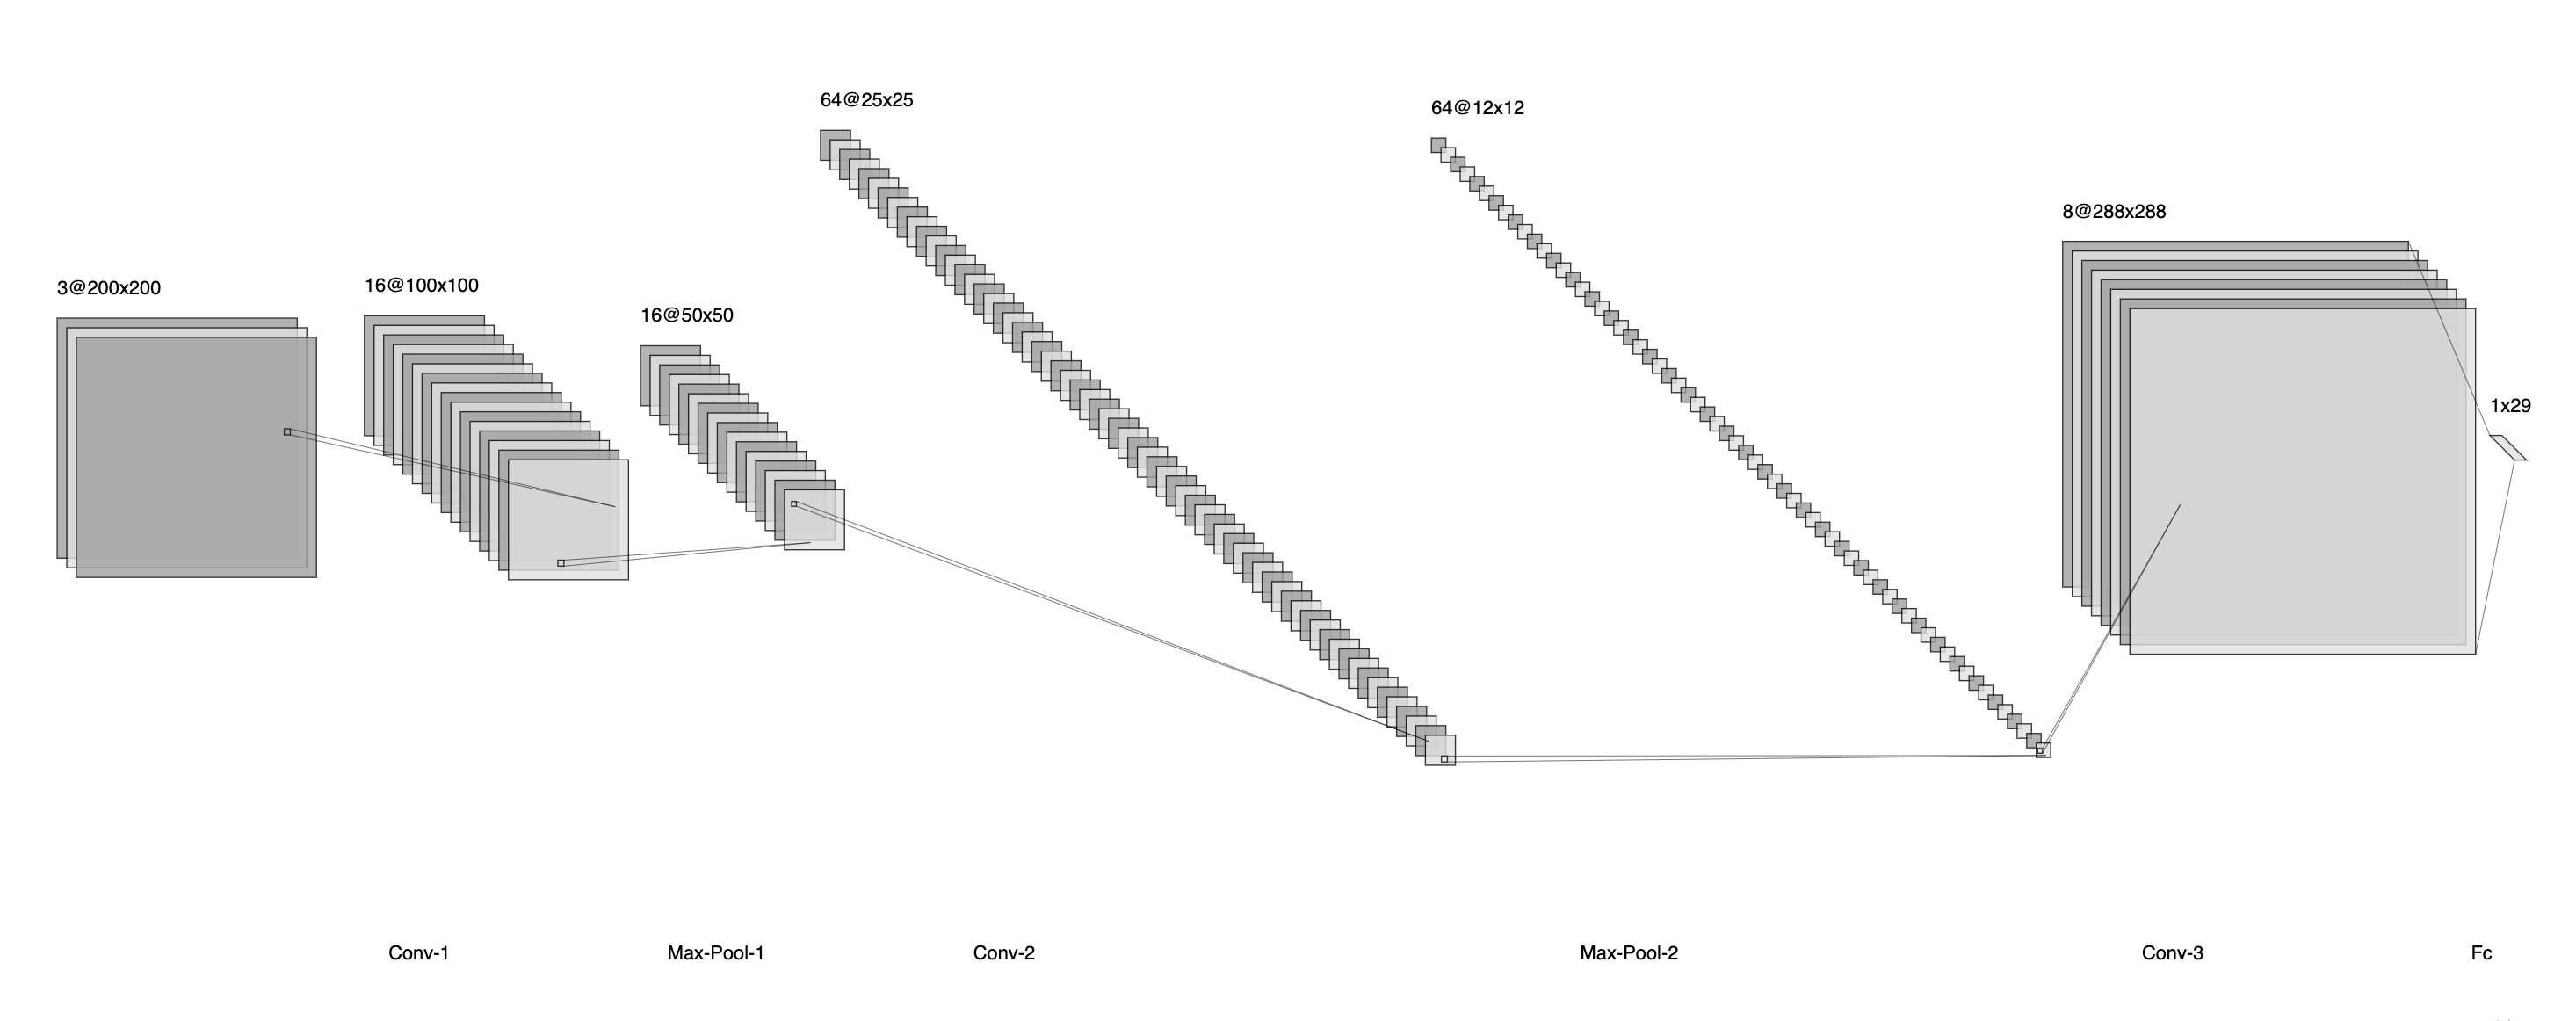
\includegraphics[width=0.43\textwidth]{../writeup_imgs/model.jpeg}

Appendix B contains the python code for our model.

\subsection{Training and Testing our Model}

We designed a Python script to train our model on the ASL dataset. We 
used PyTorch to define the model training process, including computing 
loss and evaluation. The script includes a train function that manages
the training loop and updates a plot to visualize the training process.
It is also capable of saving checkpoints after each epoch in the case
of something going wrong., saving checkpoints after each epoch, and 
updating a plot to visualize the training progress. It also includes
a testing function to assess our model's performance on a test dataset,
outputting a grid of images with the true label and predicted label.
Unfortunately, our testing dataset did not contain a test for the 
‘del’ sign, but that did not affect the testing process. 

Our main block is capable of either training the model, or restoring
our model’s training from a checkpoint. It then tests the model.

For testing, it processes images from a test set through the trained model,
and applies transformations. The transformations include resizing to
200x200 pixels, normalizing the image, and converting it to a PyTorch
\href{https://pytorch.org/docs/stable/tensors.html}{Tensor}.
This step is necessary, as the input images must be comparabl
to the images that we trained on. The output predictions are
then compared against the true labels, and the results are displayed using matplotlib. 

Our training and testing script also uses functions from another script, 
which provides useful functions for model checkpoint saving and epoch 
evaluation. These functions enable counting learnable parameters in 
a model and saving and restoring model states to resume training or 
evaluate from different stages of training. Additionally, the script 
contains functions that evaluate model performance across training, 
validation, and testing datasets, plotting metrics such as accuracy 
and loss. The train\_epoch function updates the model's weights during
training iterations, and the predictions function interprets the model’s class predictions.

Appendix C contains the python code for training and testing our model.

\subsection{Initial Testing}
With our model trained, we could test our data on a set of 28 ASL signs: A-Z, 
as well as ‘nothing’, which is simply no sign, and ‘space’ which represents 
the space character on a keyboard. Our model performed fairly well, and achieved
a testing accuracy of 78.6\%. We were satisfied with the result, but thought that we could do better.

\subsection{Data Modification}
In order to achieve higher testing accuracy than 78.6\%, we decided to modify 
each picture. Our dataset contained 250 pictures for each letter and symbol,
which meant there were 250 * 29 = 7250 files already in our dataset. It took
about 9 minutes for our model to train the first time, so we decided to only
modify 50 pictures for each letter. For data modification, we had four different
techniques: gaussian blur, grayscale, grayscale combined with gaussian Blur,
and rotation. For gaussian Blur, we used cv2’s
\href{https://docs.opencv.org/4.x/d4/d86/group__imgproc__filter.html#gaabe8c836e97159a9193fb0b11ac52cf1}{implementation}.
For grayscale, we used numpy to convert our images to a single color channel,
reducing the complexity and focusing the model on structural features. 
For rotation, we used SciPy’s
\href{https://docs.scipy.org/doc/scipy/reference/generated/scipy.ndimage.rotate.html}{rotate}
function with an angle of 20 degrees. In Appendix D, you can find the
full python code for our data modification. 
Other than using SciPy, cv2, and numpy’s libraries for certain data 
modification, the rest of the code was implemented by us. Here is an example
of an original image from the dataset (letter O), and the corresponding modified data:
\\\begin{center}
    Original: \\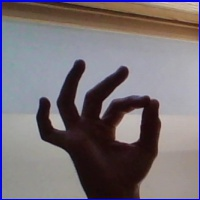
\includegraphics[width=0.43\textwidth]{../asl_alphabet_modified/F/F40.jpg}\\F40.jpg
    \vspace{3mm}
    \\\begin{tabular}{|c|c|}
        \hline
        Gaussian Blur & Grayscale \\
        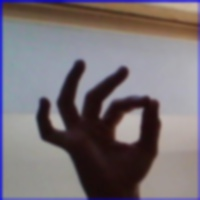
\includegraphics[width=0.18\textwidth]{../asl_alphabet_modified/F/F291.jpg}
        & 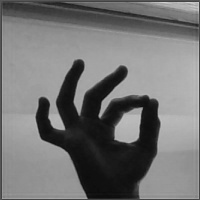
\includegraphics[width=0.18\textwidth]{../asl_alphabet_modified/F/F793.jpg} \\
        F291.jpg & F793.jpg \\
        \hline
        Gray + Gaussian & Rotation \\
        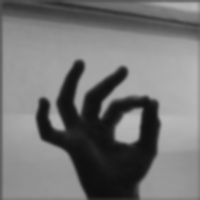
\includegraphics[width=0.18\textwidth]{../asl_alphabet_modified/F/F542.jpg}
        & 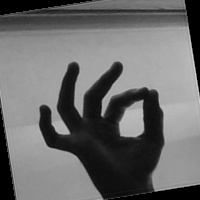
\includegraphics[width=0.18\textwidth]{../asl_alphabet_modified/F/F1044.jpg} \\
        F542.jpg & F1044.jpg \\
        \hline
    \end{tabular}
\end{center}

%-------------------------------------------------------------------------
%----------------------------------METHODOLOGY END------------------------
%-------------------------------------------------------------------------



%-------------------------------------------------------------------------
%----------------------------------RESULTS--------------------------------
%-------------------------------------------------------------------------
\section{Results}
\subsection{Training on original data}
After training our model for 5 epochs on unmodified data, our model achieved 99.0\% training accuracy,
98.2\% validation accuracy, and 97.4\% testing accuracy. In terms of loss, we achieved 0.0354 training
loss, 0.0833 validation loss, and 0.1228 testing loss. Included below is a plot of our training data.

\begin{center}
    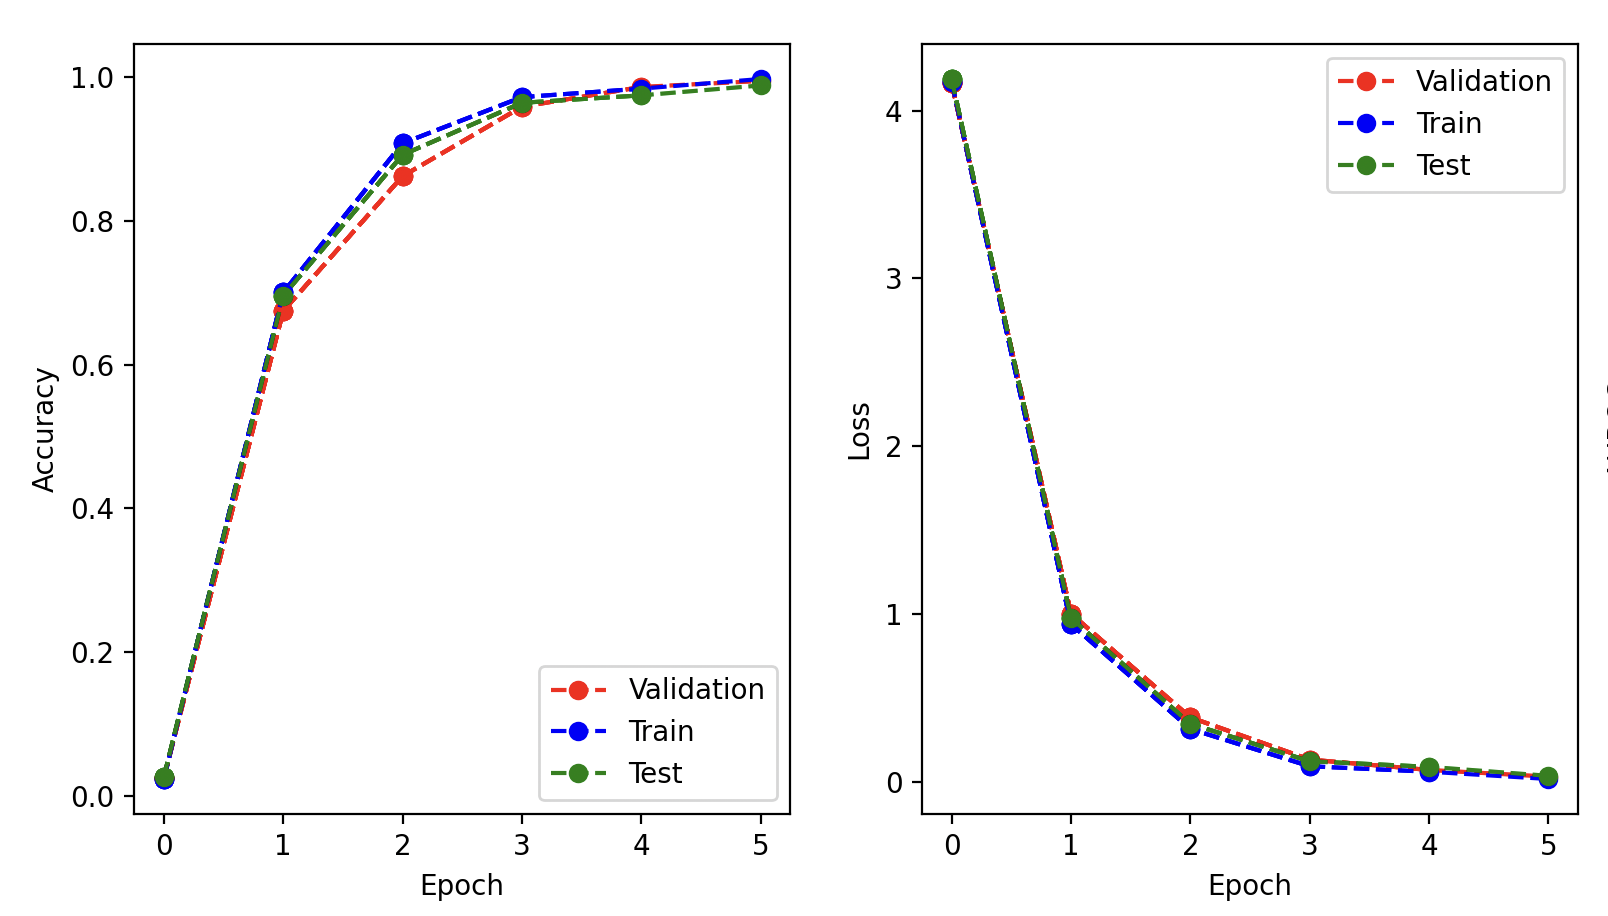
\includegraphics[width=0.43\textwidth]{../writeup_imgs/model1Plot.png}
\end{center}

\subsection{Results from testing}
After training, we could tested our data on a set of 28 ASL signs: A-Z, as well as ‘nothing’
and the ‘space’ character. Attached below is a plot of our results.

\begin{center}
    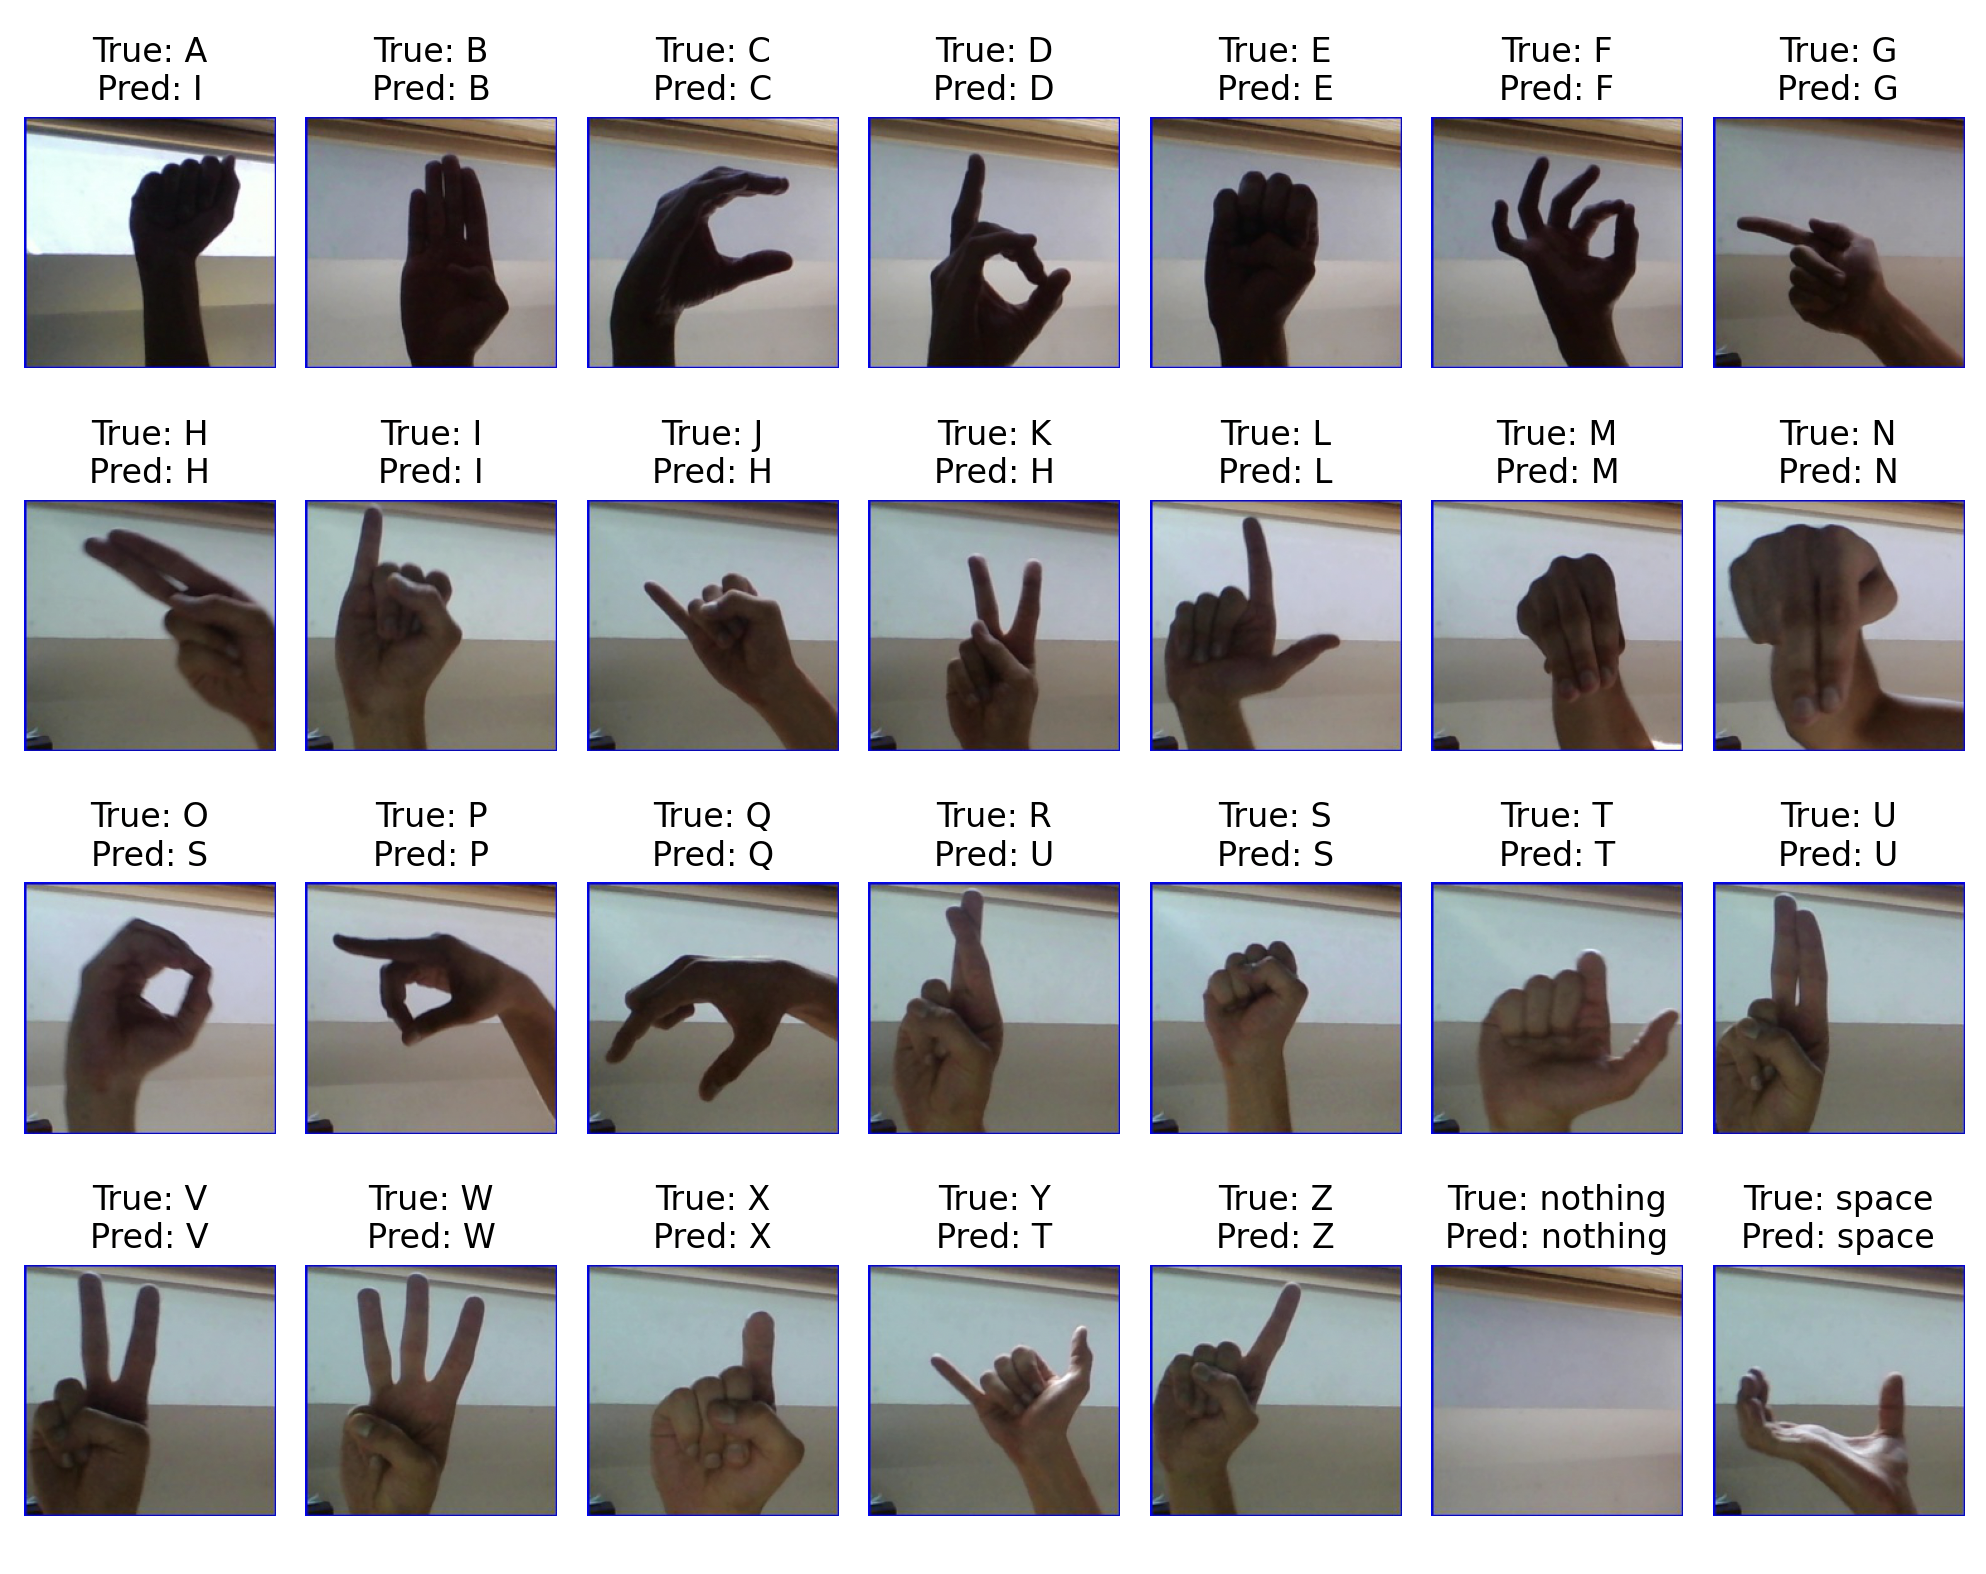
\includegraphics[width=0.43\textwidth]{../writeup_imgs/test_output.png}
\end{center}

Our model performed well, but it did not correctly predict “A”, “D”, “H”, “J”, “O”, and “Y”.
This results in a test accuracy of 78.6\%. There could be multiple reasons for
the discrepancies between the actual test accuracy of 78.6\% and the reported test accuracy of 97.4\%.
Our group concluded that the most reasonable interpretation is that the model may have overfitted to the training data,
capturing noise and specific patterns that do not work well with the actual test data. This likely led to high reported
testing accuracy, but lower performance on the real test set. We were satisfied with 78.6\% accuracy,
but thought that we could do better, and trained our model on the original data coupled with modified data.

\subsection{Training with modified data}
Training our model for 5 epochs with modified data achieved similar accuracies and losses.
With modified data, our model achieved 99.7\% training accuracy, 99.5\% validation accuracy, and 98.8\%
testing accuracy. For loss, it achieved 0.0192 training loss, 0.0332 validation loss, and 0.0381
testing loss. Below is a plot with our modified training data. 

\begin{center}
    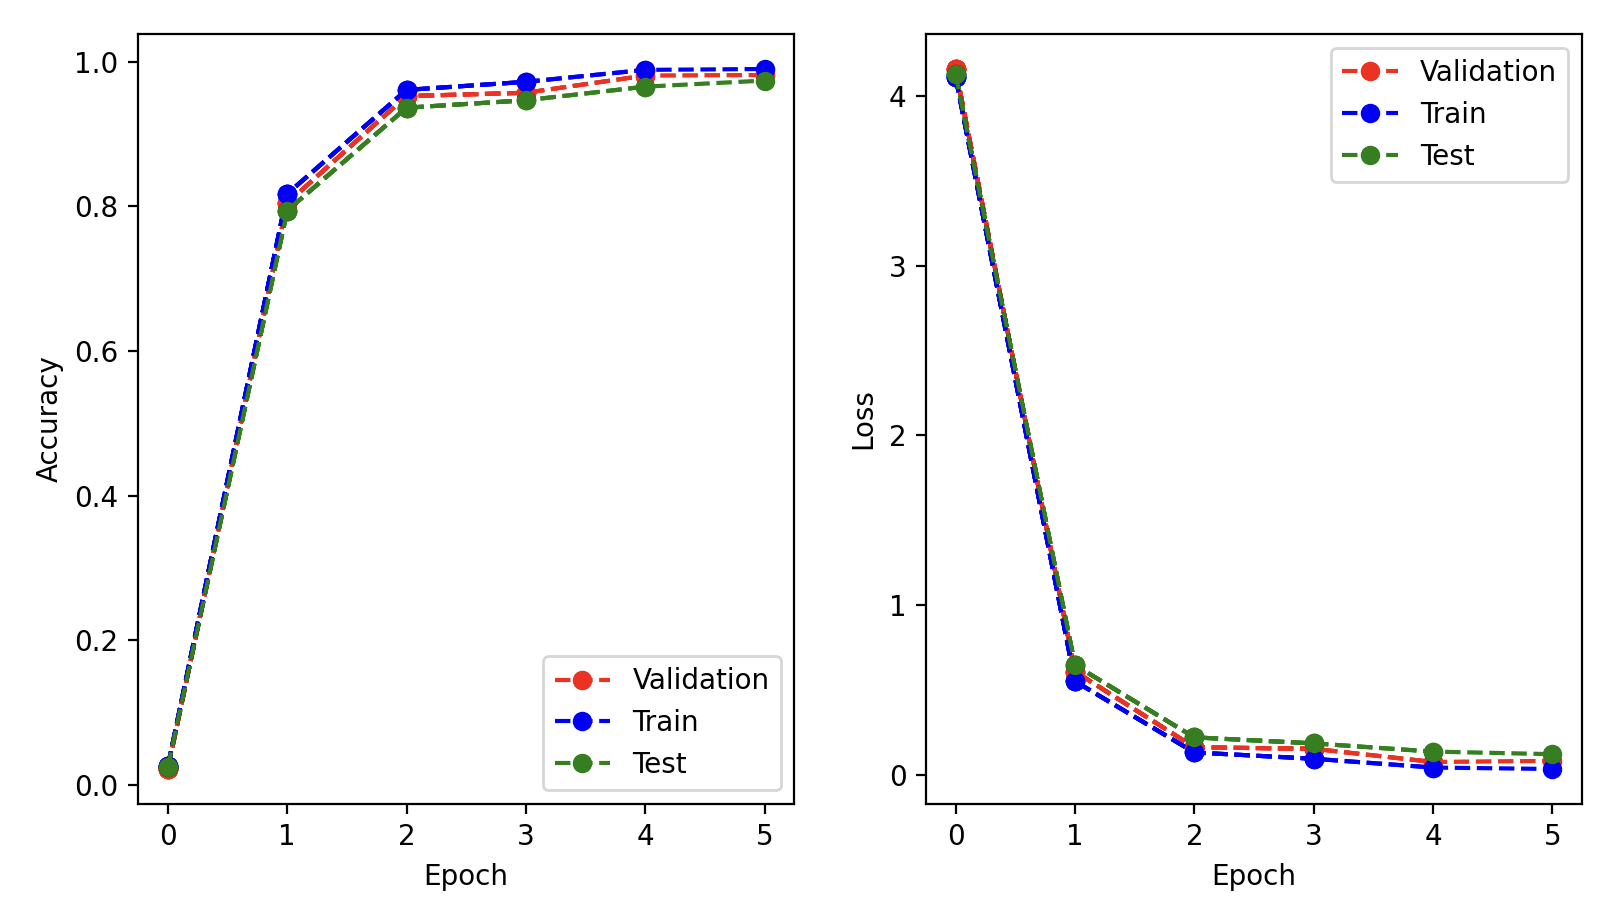
\includegraphics[width=0.43\textwidth]{../writeup_imgs/model2Plot.png}
\end{center}

Although the end result was similar, our model achieved a higher accuracy quicker 
(after the first epoch) and a smaller loss quicker. 

\subsection{Modified Data Results}
We tested our data on the same set of 28 ASL signs. Attached below is a plot of our results.

\begin{center}
    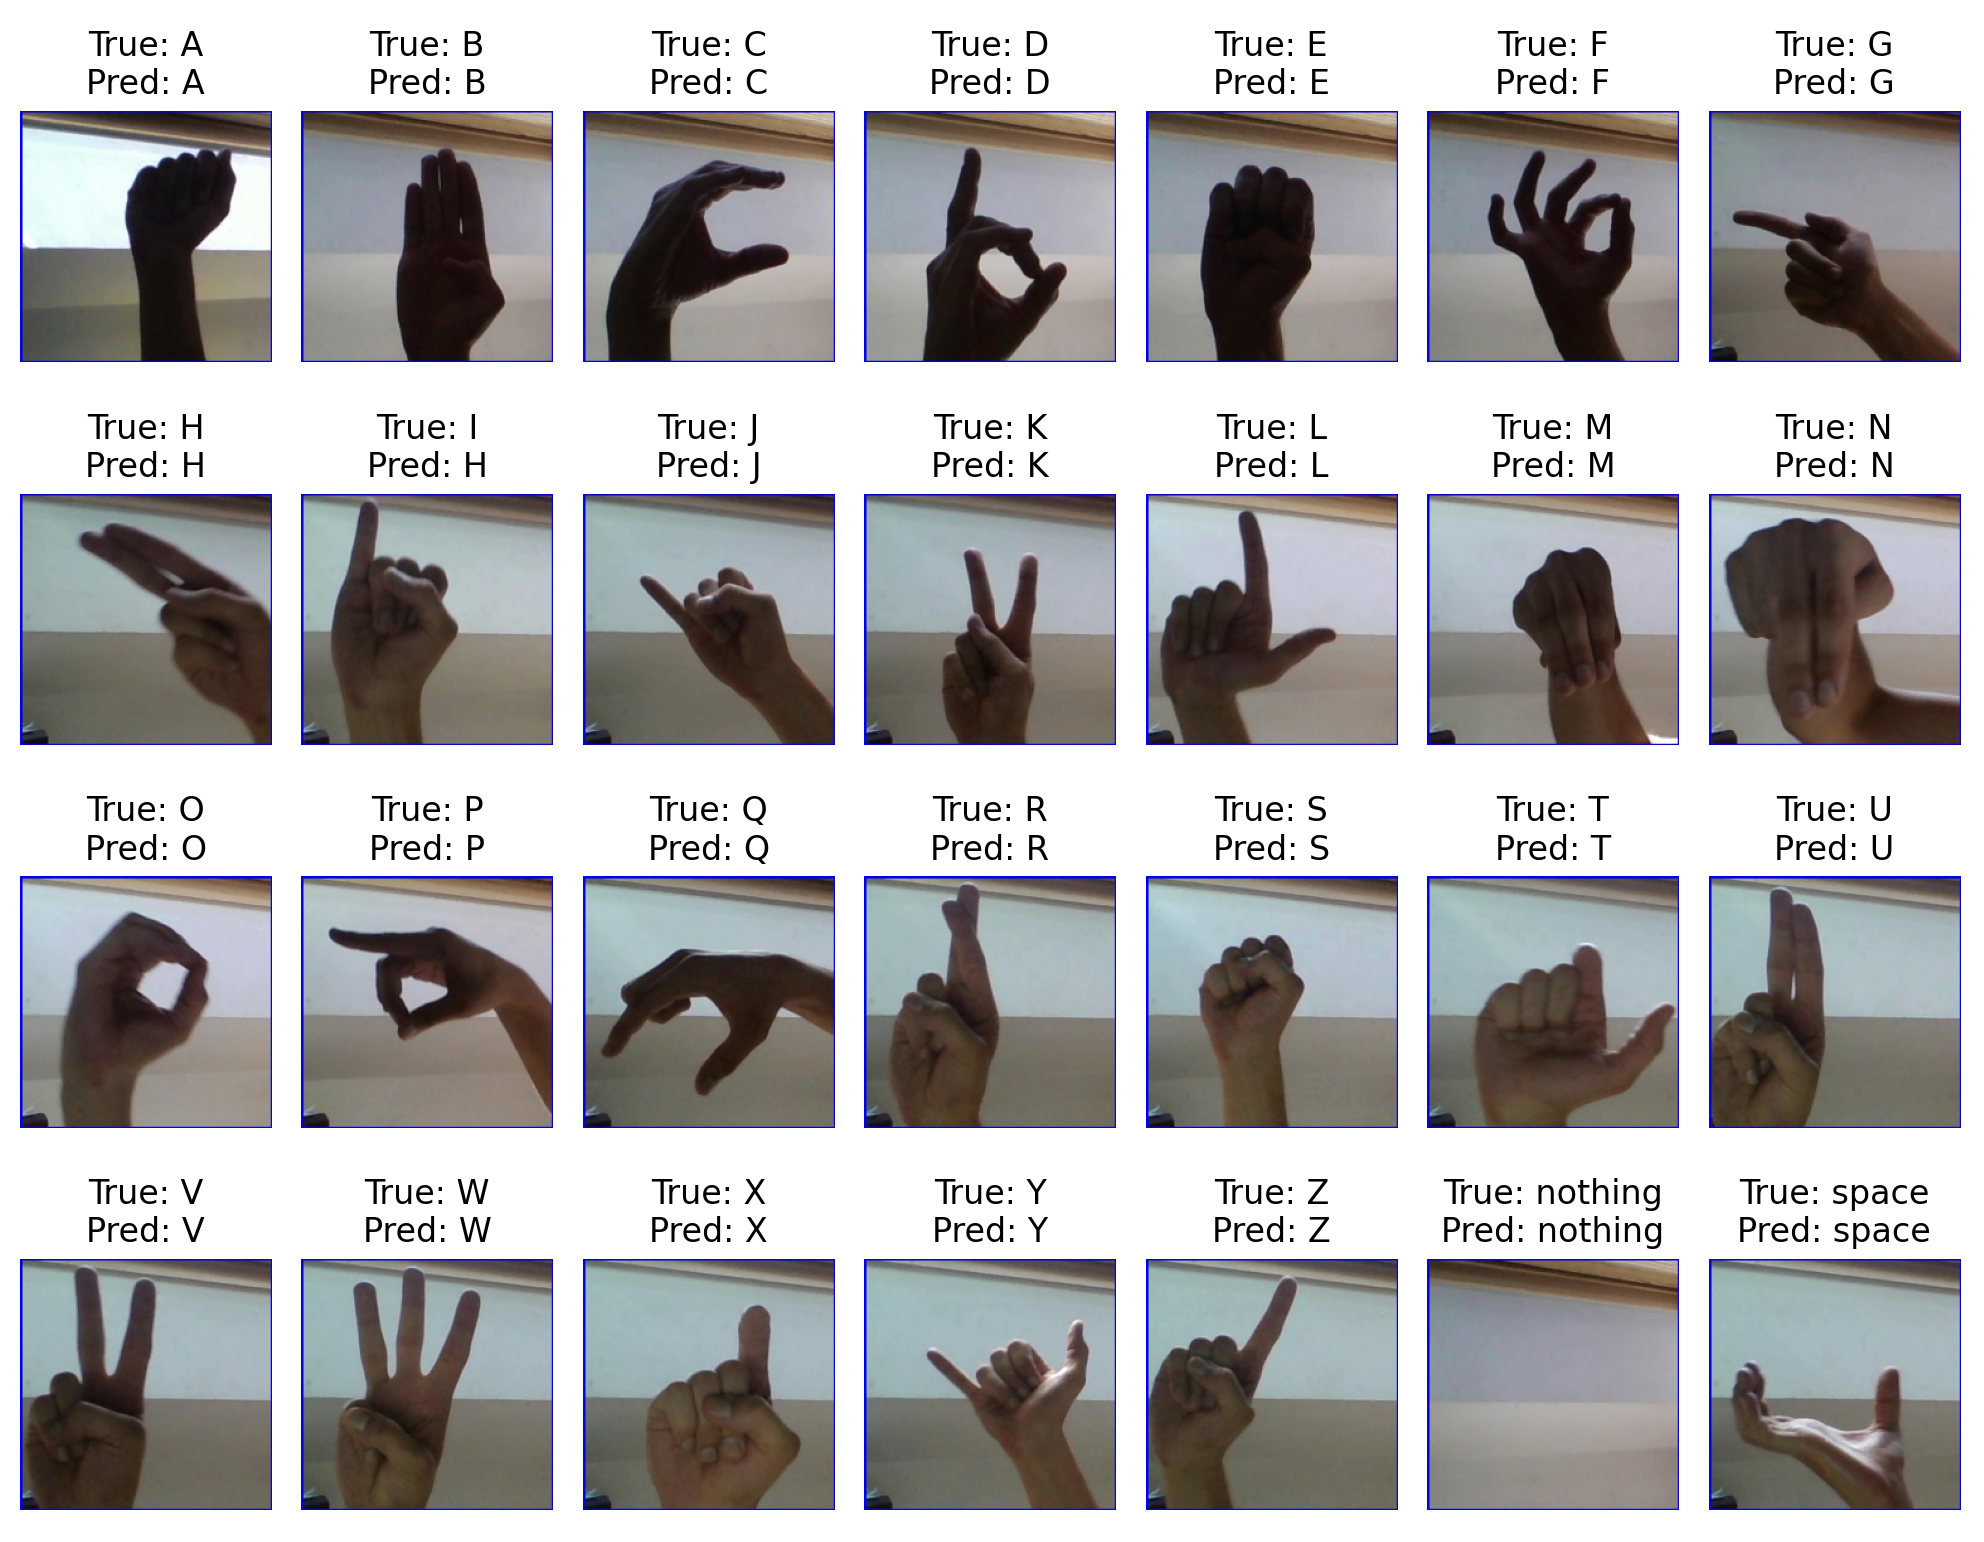
\includegraphics[width=0.43\textwidth]{../writeup_imgs/test_modified.png}
\end{center}

Our model performed better than with the original data. The only incorrect prediction was
“I”, and our model predicted it to be “H”. Thus, our test accuracy was 96.4\%, which is close
to our reported testing accuracy of 98.8\%. Modifying the data with gaussian blur, grayscale,
and rotation, counteracted the negative effects of overfitting by introducing more variability
into the dataset, which helped the model generalize better to unseen data. This result is as
predicted, as a model will perform better when it is not overfit. 

Appendix D contains code for testing data. 
%-------------------------------------------------------------------------
%----------------------------------RESULTS END----------------------------
%-------------------------------------------------------------------------



%-------------------------------------------------------------------------
%----------------------------------CONCLUSION-----------------------------
%-------------------------------------------------------------------------
\section{Conclusion}
In this project, we developed a machine learning model to identify letters and 
symbols from the American Sign Language alphabet. The model was built as a 
convolutional neural network, and trained to classify 29 ASL alphabet signs, 
including the letters A-Z and ‘nothing’ and ‘space’. This work has many possible
applications, such as automatically creating captions from sign language in 
virtual conferences or meetings, fostering more inclusive interactions. 
We trained our model with a dataset of 7250 images containing ASL signs for
A-Z, ‘nothing’, ‘space’, and ‘del’. Our model performed well, and performed
even better after we added modified images.  

If we had more time, we would have made it such that our model can predict pictures 
that we create ourselves. We did try experimenting with the model structure, 
training hyperparameters, as well as finding new data to train our model on. 
However, it was insufficient in predicting ASL signs that we created ourselves.

From this project, it is clear that data modification techniques can mitigate 
overfitting, leading to a model that generalizes better to unseen data. The 
improved performance with the modified dataset supports the idea that introducing
variability can enhance a model's predictive capabilities.

%-------------------------------------------------------------------------
%----------------------------------CONCLUSION END-------------------------
%-------------------------------------------------------------------------



%-------------------------------------------------------------------------
%----------------------------------REFERENCES-----------------------------
%-------------------------------------------------------------------------
\section{References}
{\small
\bibliographystyle{ieee_fullname}
\bibliography{egbib}
    Akash. (2018, April 22). Asl alphabet. Kaggle. https://www.kaggle.com/datasets/grassknoted/asl-alphabet 
    \\\\Coldewey, D. (2019, August 20). This hand-tracking algorithm could lead to sign language recognition. TechCrunch. https://techcrunch.com/2019/08/19/this-hand-tracking-algorithm-could-lead-to-sign-language-recognition/?guccounter=1. 
    \\\\Galario, G. (2020, July 3). Image classification on the American Sign Language Alphabet Dataset. Medium. https://medium.com/@gryangalario/image-classification-on-the-american-sign-language-alphabet-dataset-45da66f8871e.
    \\\\Garimella, M. (2022, August 23). Sign language recognition with Advanced Computer Vision. Medium. https://towardsdatascience.com/sign-language-recognition-with-advanced-computer-vision-7b74f20f3442.
    \\\\S, E. (2024, April 18). ML\_ASL\_ALPHABET: CNN model (96\% accuracy). Kaggle. https://www.kaggle.com/code/reemasolan/ml-asl-alphabet-cnn-model-96-accuracy.
}
%-------------------------------------------------------------------------
%----------------------------------REFERENCES END-------------------------
%-------------------------------------------------------------------------



%-------------------------------------------------------------------------
%----------------------------------APPENDIX-------------------------------
%-------------------------------------------------------------------------
\newpage
\section{Appendix}
\href{}{Link to github repository}

\subsection{Appendix A: Code for loading and splitting data}
Please see dataset.py in the github repository.

\subsection{Appendix B: Code for model}
Please see model.py in the github repository. 

\subsection{Appendix C: Code for training and testing}
Please see train.py and train\_common.py in the github repository.

\subsection{Appendix D: Code for data modification}
Please see datamodification.py in the github repository.

%-------------------------------------------------------------------------
%----------------------------------APENDIX END----------------------------
%-------------------------------------------------------------------------

%%%%%%%%% REFERENCES

\end{document}